%\documentclass[titlepage=false]{sl2art}
\documentclass{sl2art}

\usepackage{lipsum}
\usepackage{verbatim}
\usepackage{mathtools}

\usepackage{graphicx}
\graphicspath{{fig/}}

\declaretheorem[style=theorem]{proposition}
\declaretheorem[style=definition,sibling=proposition]{definition}

\title{sl2art, a one-and-a-half-column document class}
\author{Calvin McPhail-Snyder}
\email{calvin@sl2.site}

\subjclass[2020]{XYZ123}
\keywords{documents}


\addbibresource{sources.bib}
\begin{abstract}
  Recently there has been a lot of interest in ``widemargin'' or ``one point five column'' documents, which use a narrow text block (for readability) and a wide margin for sidenotes, figures, and citations.
\texttt{sl2art} is a document class implementing many of these ideas, based on my PhD thesis design.
\end{abstract}

\begin{document}



\maketitle
\tableofcontents

\section{Design choices}

\subsection{Margins}
The most obvious choice is the use of a relatively narrow block for the main text.
This is considered best practice: it's hard to read lines with more than about 80 characters.
For example, the \texttt{amsart} class uses a similarly-sized text block; on US letter or A4 paper this leads to quite wide margins.
The idea here is to use that otherwise wasted space for auxiliary information like citations, figures, and notes.

Frequently text blocks are computed using some sort of mathematical principle; I did not do this.
Instead, I allocated enough room in the wide margin for 2in figures, then made the rest of the page fit.
In particular, my text block is somewhat wider than that of \texttt{tufte-article}.

\subsection{Title page}
I like separate title pages, even for articles.
Currently there is support for author names, addresses (i.e.\@ affiliations unless you really want to list a postal address) and emails.
I should add keywords and MSC classes.

\subsection{Fonts and colors}
The default is to use Libertine for text and Computer Modern for math.
Here is some math:
\begin{align*}
  \int_{0}^{\infty} t^{n} e^{-t} dt
  &=
  \left.- t^{n} e^{-t} \right|_{0}^{\infty}
  +
  n \int_{0}^{\infty} t^{n-1} e^{-t} dt
  \\
  &=
  n \int_{0}^{\infty} t^{n-1} e^{-t} dt
  \\
  &= n(n-1) \cdots 1 \int_{0}^{\infty} e^{-t} dt
  \\
  &= n!
\end{align*}

I have avoided using different-sized text for headings.
Instead sections are in {\scshape small caps} and {\itshape italics} and emphasized with an {\color{accent} accent} color, by default gold.
You can change it by re-defining the color {\color{accent} \texttt{accent}}.
All hyperlinks (internal and external) are in {\color{link} \texttt{link}}.%
\note{
It is sometimes considered good practice to use a different color for internal and external links, but I had trouble picking two that didn't look bad together.
Maybe someone has an idea!
}

For diagrams or colorful equations, there is a default color palette:
\begin{center}
  \begin{tabular}{ccccc}
    {\color{slred} red} 
    &
    {\color{slyellow} yellow}
    &
    {\color{slgreen} green}
    &
    {\color{slblue} blue} 
    &
    {\color{slpurple} purple} 
  \end{tabular}
\end{center}
According to an online tool I found, these should be distinguishable even for colorblind readers, but I have not tested this yet.\note{If you have trouble telling these apart, let me know!}

\section{Features}

\subsection{Margin notes and figures}
By default we use sidenotes\note{Like this one.} instead of footnotes.
Small figures (less than 2in wide) and tables can also be placed in the margin, as in Figure \ref{fig:margin-fig-example} and Table \ref{table:margin-table-example}.
\begin{marginfigure}
  \centering
  
\includegraphics{margin-fig-example.pdf}
  \caption{A marginal figure.}
  \label{fig:margin-fig-example}
\end{marginfigure}
\begin{margintable}
  \[
    \begin{array}{c|ccc}
      n & n^2 & n^3 & n^4\\
      \hline
      1 & 1 & 1 & 1\\
      2 & 4 & 8 & 16 \\
      3 & 9 & 27 & 81 \\
    \end{array}
  \]
  \caption{A marginal table.}
  \label{table:margin-table-example}
\end{margintable}

\subsection{Figures and wide figures}
Larger figures can be set in the main text block as usual.
\begin{figure}
  \centering
  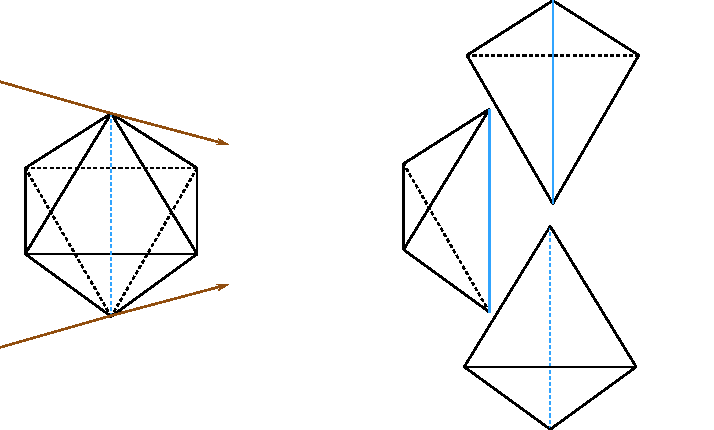
\includegraphics{fig-example.pdf}
  \caption{A larger figure.}%
  \label{fig:fig-example}
\end{figure}
For very wide figures, there is a \texttt{figure*} environment to set them across the whole page.
Unfortunately this requires some manual placement: I don't know a way to get wide figures to not overlap with marginal paragraphs automatically.
\begin{figure*}
  \centering
  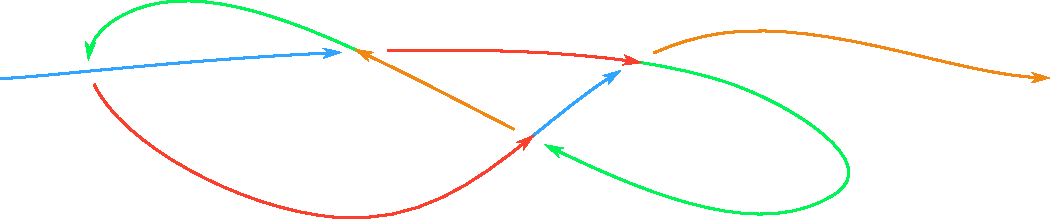
\includegraphics{wide-fig-example.pdf}
  \caption{A much larger figure.}%
  \label{fig:wide-fig-example}
\end{figure*}

\subsection{Theorems}
There is essentially one default theorem style, which looks like this:
\begin{proposition}
  Every nontrivial zero of the Riemann zeta function, the analytic continuation of
  \[
    \zeta(s) = \sum_{n=1}^{\infty} \frac{1}{n^s}
  \]
  has imaginary part \(1/2\).
\end{proposition}
There are also definitions, which don't have an end-of-statement symbol:

\begin{definition}
  A topological space \(X\) is \defemph{connected} if the only clopen sets are \(X\) and \(\emptyset\).
\end{definition}



\section{Citations}
Citations are bracketed in the text \cite{Graham1994} to match math conventions, but also go in the margin the first time they are referenced; when referenced later \cite{Graham1994} they do not produce a marginal paragraph.
This behavior is handled by the \texttt{margincite} option.


\printbibliography
  
\end{document}
